\cotefile{62}
\scanpage{36}
\begingroup\scriptsize
\diagram{\begin{tikzcd}[ampersand replacement=\&,column sep=.35em,row sep=2.6em,cramped]
t\ P^1\arrow[d,"\mathbb Z/3"',"f"]\arrow[d,phantom,"\scriptstyle\deleted{\unsure{dt''/t}}"',near end]
\&\substack{\underbrace{0,1,\infty}\\\deleted{\unsure{0,1,\infty;\,2,-1,1/2}}}\arrow[d,no head]
\&\substack{\underbrace{2,-1,1/2}\\\deleted{\unsure{2,-1,1/2}}}\arrow[d,no head]
\&\substack{x'\deleted{\unsure{x''}}=\\\tfrac12(1+\sqrt{-3})}\arrow[d,no head,shift left=.7]\arrow[d,no head,"\text{ramifié}"]\arrow[d,no head,shift right=.7]
\&{}\&\substack{x''=\\\tfrac12(1-\sqrt{-3})}\arrow[d,no head,shift left=.7]\arrow[d,no head,"\text{ramifié}"]\arrow[d,no head,shift right=.7]\\
s\ P^1\arrow[d,"\mathbb Z/2"',"g"]
\&\infty\arrow[d,no head,shift left=.5,"\text{ramifié}"]\arrow[d,no head,shift right=.5]
\&0\arrow[d,no head,shift left=.5,"\text{ramifié}"]\arrow[d,no head,shift right=.5]
\&1\deleted{\unsure{x}}\arrow[dr,no head,postaction={decorate,decoration={zigzag,segment length=4pt,amplitude=1.55pt}},"\deleted{\diagdown}"']
\&{\underbrace{\hspace{2em}}}\arrow[d,no head,"\text{non ramifié}"]
\&-1\arrow[dl,no head,postaction={decorate,decoration={zigzag,segment length=5pt,amplitude=1.1pt}},"\deleted{\diagup}"]\\
r\ P^1\&\infty\&0\&{}\&1\&{}
\arrow[from=1-2,to=2-3,phantom,pos=.58,"\substack{\text{non ramifié}\\\swarrow\quad\searrow}" description]
\end{tikzcd}}
\endgroup

Pour déterminer explicitement $f$ et $g$, on procède ainsi. [On \deleted{\illegible{1}} peut supposer que \deleted{$S=\operatorname{Spec}(\mathbb Z\deleted{\unsure{a}}[2^{-1},3^{-1}])$} \inserted{$S=\operatorname{Spec}(A)$, $A=\mathbb Z[2^{-1},3^{-1}]$} puisque \unsure{de fait|de même|de tte|toute} la situation provient par image inverse d'une situation sur $\operatorname{Spec}(A)$]. La restriction de $g$ \unsure{:|à} $P^1_S-(\infty)-(0)$ est alors un \deleted{\unsure{$S$-sch}} morphisme de $G_m$ dans lui-=, donc est de la forme $t\mathbin{\unsure{-|\to|\mapsto}}\lambda t^n$, où $n\in\mathbb Z$, et $\lambda\in\mathrm H^0(S,\underline{\mathcal O}_S^{+})$. Comme $g(\infty)=\infty$, on a $n>0$, et comme $g$ est \inserted{un rev.} d'ordre $2$, on a $n=2$. D'autre part \deleted{$\lambda$ \unsure{est une}} \inserted{$g(1)=1$, d'où $\lambda=1$}

\deleted{unité de $A$, donc de la forme $2^\alpha 3^\beta$.}

\begingroup\csname tagsleft@true\endcsname
\[
r=g(s)=s^2 \tag*{(9)}
\]
\endgroup

\uline{Cette formule est valable sur tout $P^1$} [lui donner un sens, et justifier cette assertion --- ]
% archive sheet number: 35

\scanpage{37}
\mspage{- 44 -}
n\textsuperscript{o} 272

$\Gamma_\omega/\Gamma_v$ sont finis, le groupe $\Gamma_{v'}/\Gamma_v$ est un groupe de torsion. On raisonne de même pour montrer que $L_{A'}/K_A$ est algébrique.

\uline{Corollaire} 1 - \uline{Le rang de} $v'$ \uline{est égal à celui de} $v$.

Posons pour simplifier les notations, $G=\Gamma_v,G'=\Gamma_{v'}$, et soit $S$ (resp. $S'$) l'ensemble des sous-groupes isolés de $G$ (resp. $G'$). Nous allons montrer que l 'application $H'\longrightarrow H'\cap G$ est une bijection de $S'$ sur $S$, ce qui établira évidemment que $v$ et $v'$ ont même rang. Tout d'abord, il est clair que $H'\in S'\Rightarrow H'\cap G\in S$ ; si de plus $H'_1\subset H'_2$ sont deux sous-groupes isolés de $G'$ tels que $H'_1\cap G=H'_2\cap G$, le groupe quotient $H'_2/H'_1$ est isomorphe à un sous-groupe de $G'/G$ ; comme le premier groupe est un groupe totalement ordonné et que le sedond est un groupe de torsion d'après la prop.2, il s'ensuit que $H'_2/H'_1=0$, et l'application considérée est injective. Enfin, si $H$ est un sous-groupe isolé de $G$, soit $H'\subset G'$ l'ensemble des $x\in G'$ tels qu'il existe $h\in H$ avec $-h\leq x\leq h$ ; on vérifie immédiatement que $H'$ est un sous-groupe isolé de $G'$ tel que $H'\cap G=H$, ce qui achève la démonstration.

\handwritten{[}Est-il nécessaire de dégager lo ou les lemmes sur les groupes ordonnés que l'on vient en fait de démontrer ?\handwritten{]}

\uline{Corollaire} 2 - \uline{Pour que} $v'$ \uline{soit triviale} (resp. \uline{de rang} 1), \uline{il faut et il suffit que} $v$ \uline{soit triviale} (resp. \uline{de rang} 1).

Ce sont les cas particuliers du corollaire précédent correspondant aux valeurs 0 et 1 du rang.

\uline{Corollaire} 3 - \uline{Supposons que} $L$ \uline{soit une extension finie de} $K$. \uline{Alors}, \uline{pour que} $v'$ \uline{soit discrète}, \uline{il faut et il suffit que} $v$ \uline{le soit}.

Si $v'$ est discrète, le groupe $\Gamma_v$ est isomorphe à un sous-groupe de $\uuline{Z}$, non réduit à $0$ d'après le cor.2 donc $v$ est discrète. Réciproquement, si $v$ est discrète, la prop.1 montre que $\Gamma_{v'}/\Gamma_v$ est un groupe fini, donc $\Gamma_{v'}$
% archive sheet number: 36

\scanpage{38}
On procède de $=$ pour $f$, en notant \inserted{comme dessus} qu'il ne peut exister qu'\uline{une seule $f$} : \deleted{\unsure{d'ordre|et de}} \inserted{$P^1_S\mathbin{\unsure{-|\to}}P^1_S$} définissant un \unsure{revêtem\textsuperscript{t}|revêtement} d'ordre donné (ici 3) et dont la valeur en une section (p.ex. 0) disjointe de la ramification -- \unsure{convertie|consistant} en trois sections disjointes -- soit donnée. On trouve, en ramenant \unsure{cette|la} ramification \unsure{à|:} être $0,\infty$ et \unsure{revenant|arrivant|aucune} en arrière

\begingroup\small
\[
\begin{aligned}
s=f(t)&=\frac{1+\left(\frac{\deleted{\unsure{x}}t-x'}{\deleted{\unsure{x'}}t-x''}\right)^3}
{1-\left(\frac{\deleted{\unsure{x}}t-x'}{\deleted{\unsure{x'}}t-x''}\right)^3}
=\frac{(t-x'')^3+(t-x')^3}{(t-x'')^3-(t-x')^3}\\
&=\frac{2t^3-3t^2({x''}^{\deleted{\unsure{2}}}+{x'}^{\deleted{\unsure{2}}})+3t^{\deleted{\unsure{2}}}({x'}^{2}+{x''}^{2})-({x'}^{3}+{x''}^{3})}
{3t^2(x'-x'')+3t({x''}^{2}-{x'}^{2})-({x''}^{3}-{x'}^{3})}
\end{aligned}
\]
\endgroup

\noindent\begin{minipage}[t]{.48\linewidth}\scriptsize
\tikz[overlay,baseline,x=\linewidth,y=1ex]{\draw[thin] (.06,1.8) .. controls (.31,1.6) and (.55,1.5) .. (.69,1.3) .. controls (.73,1.1) and (.74,.2) .. (.76,-.7) .. controls (.8,-1.1) and (.86,-.85) .. (.88,-2.65) .. controls (.88,-3.3) and (.93,-4.0) .. (.95,-4.25) .. controls (.97,-4.6) and (1,-5.7) .. (1,-6.55) .. controls (1.04,-9.5) and (.99,-10.5) .. (1.015,-13) .. controls (1.045,-17.8) and (1.005,-23.5) .. (1.02,-30);}
\diagram{\begin{tikzcd}[ampersand replacement=\&,column sep=6em,row sep=4.5em]
\substack{\infty\\(x',x'')\deleted{\unsure{x}}\\P^1} \arrow[r,leftrightarrow,"u"{below},"{u^*(t)=\frac{t-x'}{t-x''}}"] \arrow[d,"f"] \& \substack{1\\(0,\infty)\\P^1} \arrow[d,"{h^*(t)=-t^3}"] \\
\substack{P^1\\(1,-1)\\\infty} \arrow[r,"v","{v^*(t)=\frac{1-t}{1+t}}"'] \& \substack{P^1\\(0,\infty)\\-1} \arrow[l,shift left=3.5,"{v^{-1*}(t)=\frac{1-t}{1+t})}"]
\end{tikzcd}}

\[
\begin{aligned}
f&=v^{-1}hu\\
f^*(t)&=u^*h^*v^{-1*}(t)=u^*h^*\left(\frac{1-t}{1+t}\right)\\
&=u^*\frac{1-h^*t}{1+h^*t}\mathbin{\unsure{=|:}}u^*\frac{1+t^3}{1-t^3}\\
&=\frac{1+u^*(t)^3}{1-u^*(t)^3}=
\end{aligned}
\]
\end{minipage}\hfill\begin{minipage}[t]{.47\linewidth}\scriptsize
Or ($x'$ et $x''$ étant racines pri\uline{mitives} $6^{\unsure{\text{èmes}|\text{ièmes}}}$ de 1)
\[
\begin{aligned}
{x'}^{3}={x''}^{3}&=-1,\quad\text{d'où}\quad {x''}^{3}-{x'}^{3}=0\\
\left\{\begin{array}{l}x'+x''=1\\x'x''=1\end{array}\right.&\\
{x'}^{2}+{x''}^{2}&=(x'+x'')^2-2x'x''=-1\\
(x'-x'')^2&=(x'+x'')^2-4x'x''=-3\\
x'-x''&=\sqrt{-3}\\
{x''}^{2}-{x'}^{2}&=(x''-x')(x''+x')=-\sqrt{-3}\\
\deleted{{x''}^{3}-{x'}^{3}=(x''-x')({x''}^{2}+x'x''+{x''}^{\unsure{2}})=\unsure{\sqrt{-3}(|-\sqrt{-3}(}}&
\end{aligned}
\]
\[
\begin{aligned}
f(t)&=\frac{1}{3\sqrt{-3}}\frac{2t^3-3t^2-3t+2}{t(t-1)}\\
&=\frac{1}{3\sqrt{-3}}\frac{(t+1)(2t-1)(t-2)}{t(t-1)}
\end{aligned}
\]
\end{minipage}
% archive sheet number: 37

\scanpage{39}
\mspage{- 43 -}
n\textsuperscript{o} 272

dans $A'$ des éléments $y_\alpha$ ($\alpha=1,\ldots,s$) dont les images $\bar y_\alpha$ dans $L_{A'}$ sont linéairement indépendantes sur $K_A$ ; on a évidemment $v'(y_\alpha)=0$ pour tout $\alpha$. Nous allons montrer que les éléments $x_i y_\alpha$ sont linéairement indépendants sur $K$, ce qui établira bien l'inégalité $rs\leq n$.

Supposons donc qu'il existe une relation linéaire non triviale de la forme ;
\begingroup\csname tagsleft@true\endcsname
\[
\sum a_{i\alpha}x_i y_\alpha=0\quad,\ a_{i\alpha}\in K. \tag*{(2)}
\]
\endgroup

Soit $a_{j\beta}x_j y_\beta$ celui des termes de (2) dont la valuation est minimum ; on a donc $v'(a_{i\alpha}x_i y_\alpha)\geq v'(a_{j\beta}x_j y_\beta)$ pour tout couple $(i,\alpha)$ ; si $i\ne j$, on ne peut avoir égalité, car cela entraînerait
\begingroup\csname tagsleft@true\endcsname
\[
v'(x_i)-v'(x_j)=v'(a_j)-v'(a_i)\qquad\equiv 0\ \mathrm{mod.}\ \Gamma_v, \tag*{(3)}
\]
\endgroup
contrairement au choix des $x_i$. On a donc :
\[
v'(a_{i\alpha}x_i y_\alpha)>v'(a_{j\beta}x_j y_\beta)\qquad\text{pour } i\ne j
\]

En multipliant la relation (2) par $(a_{j\beta}x_j)^{-1}$ et en posant $b_\alpha=a_{j\alpha}\cdot a_{j\beta}^{-1}$ on obtient alors une relation de la forme :
\begingroup\csname tagsleft@true\endcsname
\[
\sum b_\alpha y_\alpha+z=0\quad,\ \text{avec }v'(b_\alpha)\geq 0,\ v^{\unsure{\prime|:}}(z)>0, \tag*{(4)}
\]
\endgroup
d'où, dans $L_{A'}$, une relation :
\begingroup\csname tagsleft@true\endcsname
\[
\sum\bar b_\alpha\bar y_\alpha=0. \tag*{(5)}
\]
\endgroup

Comme $b_\beta=1$, ceci contredit l'hypothèse faite sur les $y_\alpha$, et achève la démonstration.

PROPOSITION 2 - \uline{Supposons que} $L$ \uline{soit une extension algébrique de} $K$. \uline{Alors le groupe quotient} $\Gamma_{v'}/\Gamma_v$ \uline{est un groupe de torsion}, \uline{et l'extension} $L_{A'}/K_A$ \uline{est une extension algébrique}.

Soit $\{L_\omega\}$ la famille des extensions finies de $K$ contenues dans $L$, et soit $\Gamma_\omega=v'(L_\omega^*)$. Le groupe $\Gamma_{v'}$ est réunion de la famille filtrante croissante formée par les $\Gamma_\omega$ ; comme, d'après la prop.1; les groupes
% archive sheet number: 38

\scanpage{40}
On obtient ainsi
\begingroup\csname tagsleft@true\endcsname
\[
f(t)=\frac{1}{3\sqrt{-3}}\frac{(t+1)(2t-1)(t-2)}{t(t-1)} \tag*{(10)}
\]
\endgroup
et par suite
\[
\boxed{\unsure{\rho^*(t)|p^*(t)}=(gf)^*(t)}\!\boxed{=j=\frac{1}{-27}\left(\frac{(t+1)(2t-1)(t-2)}{t(t-1)}\right)^2} \tag*{(11)}
\]

Cette formule, comme il se doit est définie sur $S$ lui-$=$, et non seulement sur $\unsure{\bar S|J|S|T|S'}$ ! Elle définit un revêtement galoisien de groupe $\mathfrak S_3$ de \deleted{$\unsure{(G_a)_S}$} $P^1_S$, \inserted{à partir de $(G_a)_S$,} qui est non ramifié au dessus de $(G_a)_S-(0)-(1)=(G_m)_S-1$.

\figure{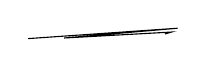
\begin{tikzpicture}[x=1em,y=1ex]\draw[thin] (-3,-.17)--(2.4,.7)--(-1.7,-.12)--(2.18,.38)--(1.94,.22);\end{tikzpicture}}

Comment opère $\sigma$ dans les quotients ?

\noindent\begin{minipage}[t]{.21\linewidth}\vspace{0pt}\scriptsize
\diagram{\begin{tikzcd}[ampersand replacement=\&,row sep=1.3em]
\sigma\quad P^1\arrow[d,"f"]\\
\sigma'\quad P^1\arrow[d,"g"]\\
\sigma''\quad P^1
\end{tikzcd}}
\end{minipage}\hfill\begin{minipage}[t]{.74\linewidth}\vspace{0pt}

On voit que $\sigma'(\infty)=0$, $\sigma'(0)=\infty$, $\sigma'(1)=1$, \deleted{d'où} $=$s formules pour $\sigma''$, d'où \deleted{$\sigma'(t)=1/t$}

\deleted{et d'autre part}
\begingroup\csname tagsleft@true\endcsname
\[
\sigma'(t)=\sigma''(t)=1/t \tag*{(11)}
\]
\endgroup
et il serait facile de passer au quotient par $\sigma$ \deleted{\unsure{de}} en dernier lieu (p.ex.).
\end{minipage}
\figure{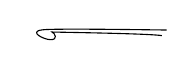
\begin{tikzpicture}[x=1em,y=1ex]\draw[thin] (2.35,.35) .. controls (1.85,.36) and (-1.8,.5) .. (-2.15,.36) .. controls (-2.65,.21) and (-2.08,-.46) .. (-1.85,-.46) .. controls (-1.55,-.48) and (-1.69,.1) .. (-1.79,.18) .. controls (-.18,.11) and (1.78,.02) .. (2.18,-.12);\end{tikzpicture}}
% archive sheet number: 39

\scanpage{41}
\mspage{- 18 -}
n\textsuperscript{o} 276

un module filtré $(E,E_n)$ sur un anneau filtré $(A,A_n)$, et soit $\hat E$ le complété du groupe abélien $E$ muni de la topologie associée à la filtration donnée $\hat E$ est donc un groupe topologique abélien, d'ailleurs métrisable puisque la topologie de $E$ est définie par un écart. Comme les sous-groupes $E_n$ forment un système fondamental de voisinages de $0$ dans $E$, \uline{les sous-groupes} $\hat E_n$ \uline{forment de même un système fondamental de voisinages de} $0$ \uline{dans le groupe} $\hat E$ et si $F$ est un sous-groupe de $E$, muni de la topologie induite, le complété de $E/F$ n'est autre que $\hat E/\hat F$. Prenant $F=E_n$ et observant que, $E_n$ étant ouvert, le quotient $E/E_n$ est discret et donc complet, on voit que \uline{les homomorphismes canoniques}
\[
E/E_n\longrightarrow\hat E/\hat E_n
\]
\uline{sont bijectifs}. On notera d'autre part que, $E_n$ étant fermé, on a, lorsque $E$ est séparé (i.e. se plonge biunivoquement dans $\hat E$), la relation
\[
E_n=E\cap\hat E_n\quad.
\]

Considérons plus particulièrement l'anneau filtré $(A,A_n)$ lui-même ; Alors $\hat A$ est un \uline{anneau topologique} (\uline{Top.Gén}. Chap.III, \S\,5, n\textsuperscript{o}4) et les relations $A_p A_q\subset A_{p+q}$ conduisent aux relations $\hat A_p\hat A_q\subset\hat A_{p+q}$ ; les sous-groupes $\hat A_p$ définissent donc une filtration de l'anneau $\hat A$, et comme ils forment un système fondamental de $0$ on voit que la topologie de $A$ est précisément définie par cette filtration. Autrement dit, \uline{le complété de l'anneau filtré} $(A,A_n)$ \uline{est l'anneau filtré} $(\hat A,\hat A_n)$. Comme de plus $\hat A/\hat A_n$ s'identifie canoniquement à $A/A_n$ il est clair que \uline{les anneaux gradués associés} $G(A)$ \uline{et} $G(\hat A)$ \uline{sont canoniquement isomorphes},

Revenant à un module filtré $(E,E_n)$ sur l'anneau filtré $(A,A_n)$, la loi de composition $A\times E\longrightarrow E$ se prolonge en une loi de composition $\hat A\times\hat E\longrightarrow\hat E$ on vérifie immédiatement qu'elle fait de $\hat E$ un $\hat A$-module ; comme de plus les
% archive sheet number: 40

\scanpage{42}
Soit $S$ un schéma de base, et soit $X$ un schéma de Br. Severi sur $S$ muni d'une \uline{trisection} non ramifiée $X'$, i.e un sous-schéma \inserted{fermé} de $X$ qui est non ramifié sur $X$, d'ordre 3 sur $X$.

Un tel truc peut être considéré comme un objet à schéma structural $\mathfrak S_3$, opérant sur $P^1_S$ comme il a été dit. La classification de tels objets est donc la $=$ que la classification des \deleted{\unsure{rev}} $\mathrm H^1(S,\mathfrak S_3)$ des \unsure{revêtem\textsuperscript{ts}|revêt\textsuperscript{ts}|rev.} \inserted{gal} \uline{non ramifiés} de \deleted{\unsure{schéma}} groupe $\mathfrak S_3$ de $S$. De plus, \unsure{on|$\sigma$} définit dans $X$ un $S$-automorphisme \inserted{involutif}, noté $\sigma$, qui transforme $X'$ en un $X''$, dit \uline{associé} à \unsure{$X$!|$X'$.|$X'$!} \unsure{Évidemt|Évidemment}, si on \unsure{partait|partant} de $(X,X'')$, on aurait le $=$ $\sigma$, et on \unsure{réobtient|restitue|trisection} $X'$ [à préciser --- ]. De plus, on obtient [par descente --- ] une \uline{bisection}, non ramifiée \deleted{[\unsure{du moins}} \unsure{en les pts|sur les pts} de $S$ de car. $\ne 2,3$]..... On peut passer au quotient, \deleted{\unsure{qui}} par $\mathfrak S_3$, \deleted{\unsure{pour}} on trouve \unsure{que|pour} :
\[
P^1_S\xrightarrow{p}P^1_S
\]
(\unsure{comp. au|lorsque} $\mathfrak S_3$ \unsure{opérant|opère}
% archive sheet number: 41

\scanpage{43}
\mspage{- 17 -}
n\textsuperscript{o} 276

\[
w:\widehat{E/F}\longrightarrow\widehat{\hat E/\hat F}
\]
Il est clair que $w\circ v$ n'est autre que l'application canonique de $\hat E/\hat F$ dans son complété ; si de plus l'on prolonge $v$ en une représentation
\[
\hat v:\widehat{\hat E/\hat F}\longrightarrow\widehat{E/F}
\]
alors $\hat v\circ w$ est l'identité, puisque c'est déjà l'identité sur $E/F$.

\uline{Si} $\hat E/\hat F$ \uline{est complet}, il résulte de ce qui précède que $v$ et $w$ sont des représentations inverses l'une de l'autre, autrement dit que $v$ est un isomorphisme du groupe topologique $\hat E/\hat F$ sur le groupe topologique $\widehat{E/F}$. D'après la prop.4, de \uline{Top. Gén}. Chap.IX, \S3, ce sera toujours le cas si le groupe $E$ est \uline{métrisable} puisqu'alors $\hat F$ est un sous-groupe fermé du groupe métrisable et complet $\hat E$. Il en sera de même plus généralement si la topologie de $E$ peut être définie à l'aide d'un écart.

On déduit de là le résultat suivant :

\uline{Lemme} 1 - \uline{Soient} $E,F,G$ \uline{trois groupes topologiques abéliens métrisables}, $u:E\longrightarrow F$ \uline{et} $v:F\longrightarrow G$ \uline{deux homomorphismes topologiques telle que la}
% slanted
\margin{\handwritten{\unsure{topolog|topolog\textsuperscript{t}|topologiques}}}\uline{suite de groupes abéliens} $E\xrightarrow{u}F\xrightarrow{v}G$ \uline{soit} \handwritten{\tikz[overlay,baseline]{\draw[thin] (0.12em,-0.42ex) .. controls (0.65em,-0.85ex) and (2.65em,-0.68ex) .. (2.87em,-0.34ex) .. controls (2.93em,-0.25ex) and (2.89em,-0.15ex) .. (2.80em,-0.12ex);}}\uline{exacte}. \uline{Alors} $\hat u:\hat E\to\hat F$ \uline{et} $\hat v:\hat F\longrightarrow\hat G$ \uline{sont des homomorphismes topologiques et la suite} $\hat E\xrightarrow{\hat u}\hat F\xrightarrow{\hat v}\hat G$ \uline{est exacte}\unsure{,|.}

On a vu en effet, que le lemme 1 est vrai lorsque $u$ est injectif et $v$ surjectif. Or dans le cas général, la suite exacte donnée se décompose en suites exactes partielles.
\[
N\longrightarrow E\longrightarrow I\ ;\ I\longrightarrow F\longrightarrow J\ ;\ J\longrightarrow G\longrightarrow K
\]
qui rentrent dans ce cas particulier, et auxquelles le lemme 1 est donc applicable ; d'où évidemment le résultat cherché puisque le composé de deux homomorphismes est un homomorphisme.

Ces préliminaires sur les groupes topologiques étant rappelés, considérons
% archive sheet number: 42

\scanpage{44}
trivialement sur le deuxième facteur) un morphisme naturel [aux \uline{pts de \uuline{car. $\ne2,3$}}]
\[
X\xrightarrow{j}P^1_S
\]
qui est ramifié en les sections $0$\deleted{$\unsure{1}$}, $\infty,1$ \deleted{\unsure{et}} exclusivement : l'image inverse de $\infty$ étant $X'$, \inserted{\unsure{ensemblist\textsuperscript{t}|ensemblistement}} celle de $\infty$ étant $X''$, celle de $1$ \deleted{étant} $X_1$.

\figure{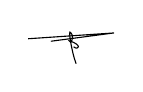
\begin{tikzpicture}[x=1em,y=1em]\draw (-1.6,0.04) -- (1.5,0.25) -- (-0.78,-0.05);\draw (0.13,-0.86) .. controls (-0.02,-0.48) and (-0.17,0.42) .. (-0.07,0.27) .. controls (0.1,0.09) and (-0.09,-0.19) .. (-0.11,-0.04) .. controls (0.38,-0.18) and (0.21,-0.40) .. (0.04,-0.25);\end{tikzpicture}}

Supposons maintenant que de plus, nous nous donnions une section $s$ de $X$ \deleted{\unsure{par}} sur $S$, ne rencontrant pas $X'$ (i.e. une section de $X-X'$ sur $S$). Son image par $j$ est alors une section de $P^1_S-(\infty)$\deleted{\unsure{,|0}}, i.e. une section de $\underline{\mathcal O}_S$, \unsure{appelé|appelée} \uline{l'invariant} de $(X,X',\deleted{\unsure{j}}s)$, soit $\deleted{j}i$

Supposons que l'invariant $\deleted{j}i$ ne prenne nulle part les valeurs $0,1$ i.e. soit inversible, ainsi que $\deleted{j}i-1$. Alors \unsure{sché|sch\textsuperscript{é}} image inverse dans $P^1_S$\deleted{$\unsure{X}$} de $p:S\to P^1_S$ définit un \deleted{section} \inserted{revêt\textsuperscript{mt}} \uline{galoisien} \uline{de} $S$, \uline{non ramifié}, \uline{de groupe} $\mathfrak S_3$, \deleted{\unsure{ici}} \uline{et c'est celui qui définit} $X$. [À \unsure{déduire les fonct\textsuperscript{is}|décrire les fonct\textsuperscript{is}|discuter les problèmes}
% archive sheet number: 43

\scanpage{45}
\mspage{- 16 -}
n\textsuperscript{o} 276

En effet, utilisons la filtration de $U(g)$ définie au n\textsuperscript{o}2, Exemple 3 ; elle est discrète : $U(g)$ est donc un anneau filtré séparé et complet ; or l'anneau gradué associé est un quotient d'un anneau de polynômes sur $K$, donc est noethérien ; d'où le corollaire.

7. - \uline{Complété d'un module filtré}.

Soit $E$ un groupe topologique abélien. Rappelons (Top. Gén..;) que le complété $\hat E$ de l'espace uniforme $E$ est canoniquement muni d'une structure de groupe abélien, et que l'application canonique de $E$ dans $\hat E$ est une \uline{représentation} du groupe topologique $E$ dans le groupe topologique $\hat E$, dont le noyau est l'adhérence de $0$ dans $E$.

Etant donné une \uline{représentation} $u$ de $E$ dans un groupe topologique abélien $E'$, l'application $u$ est uniformément continue, et par suite se prolonge en une application $\hat u:\hat E\longrightarrow\hat E'$ ; celle-ci est encore une \uline{représentation}

En particulier, soit $F$ un sous-groupe de $E$; l'application identique $j:F\longrightarrow E$ se prolonge en une représentation $\hat j$ du complété $\hat F$ dans le complété $\hat E$, laquelle est en fait un isomorphisme topologique de $\hat F$ sur un sous-groupe fermé de $\hat E$, à savoir l'adhérence de l'image de $F$ par l'application canonique de $E$ dans $\hat E$ ; nous identifierons\handwritten{\textbar}toujours $\hat F$ à son image dans $\hat E$.

Considérons de plus le groupe topologique quotient $H=E/F$ ; la représentation canonique $E\xrightarrow{u}H$ se prolonge en une représentation $\hat E\xrightarrow{\hat u}H$, et comme $u$ applique $F$ sur $e$ il est clair que $\hat u$ applique $\hat F$ sur $e$ ; donc $\hat u$ définit par passage au quotient une représentation canonique
\[
v:\hat E/\hat F\longrightarrow\widehat{E/F}\ .
\]
On a d'autre part, à partir des représentations canoniques $E\longrightarrow\hat E$ et $F\longrightarrow\hat F$, une représentation $E/F\longrightarrow\hat E/\hat F$ et par suite une représentation
% archive sheet number: 44

\scanpage{46}
catégoriques généraux --- ].

Donc en ce cas, l'invariant suffit à réconstituer \deleted{\unsure{toute|tout}} la \unsure{structure|situation} $(X,X',s)$.

Dans le cas où $X$ est normal, intègre, et où $i$ n'\uline{est pas identiquement égal} \uline{à $0$ ou $1$}, comme on \unsure{connaîtra|connaît} \unsure{le|la} \unsure{revê|couv.|revêtement}\deleted{\unsure{t|ts}} non ramifié de $X$ sur l'ouvert \inserted{$U$} où $i$ et $i-1$ inversibles $[\unsure{D_{i(i-1)}|D_{i,i-1}|S_{i(i-1)}|S_{j(j-1)}}]$, on \unsure{le|la} \unsure{connaîtra|connaît} partout, d'où reconstitution de $(X,X')$ ; d'autre part, on connaît $s$ sur $U$, donc ($X$ normal) partout.

Donc ici encore, \uline{$i$ permet de tt réconstruire}. Ici cependant, \unsure{se} pose la question : quels $i$ conviennent ??

Il faut exprimer (i) qu'une certaine extension de corps -- de degré $3$ -- du corps des fonctions de $X$ est non ramifié sur $X$ (ii) Qu'une certaine application rationnelle de $X$ qui s'en déduit est partout définie ----
% archive sheet number: 45

\scanpage{47}
\mspage{- 15 -}
n\textsuperscript{o} 276

linéaire des $\alpha_{rs}X^r$ si $r\leq n$, et des $\alpha_{ns}X^r$ si $r>n$, d'où évidemment notre assertion.

(La démonstration précédente ne semble pas présenter d'avantage très décisif par rapport à la démonstration classique \ldots)

\uline{Corollaire} 1 - \uline{Soit} $K$ \uline{un corps} ; \uline{l'anneau de polynômes} $K[X_1,..,X_r]$ \uline{est noethérien}.

On raisonne par récurrence sur $r$.

\margin{\handwritten{?}}\uline{Corollaire} 2 - \uline{Soit} $A$ \mbox{\settowidth{\unitlength}{un anneau commutatif noethérien,}\handwritten{\tikz[overlay,baseline,x=\unitlength,y=1ex]{\draw[thin] (.18,1.55) .. controls (-.1,1.2) and (-.025,-.68) .. (.16,-.62) .. controls (.52,-.37) and (.64,-1.42) .. (.86,-.99) .. controls (1.15,-.47) and (1.09,1.60) .. (.76,1.75);}}\uline{un anneau commutatif noethérien},} \uline{L'anneau de séries formelles} $A[[X]]$ \uline{est noethérien}.

Filtrons $A[[X]]$ par les puissances de l'idéal $(X)$ ; on obtient un anneau séparé et complet (Corollaire de la Proposition 5) ; or l'anneau gradué associé, isomorphe à $A[X]$, est noethérien ; donc $A[[X]]$ est noethérien en vertu du corollaire 2 de la proposition 7.

\uline{Corollaire} 3 - \uline{Soit} \mbox{\settowidth{\unitlength}{$K$ un corps ;}\handwritten{\tikz[overlay,baseline,x=\unitlength,y=1ex]{\draw[thin] (0,.47) .. controls (-.10,1.75) and (.79,2.25) .. (1.01,1.36) .. controls (1.23,.2) and (.99,-.93) .. (.64,-1.01) .. controls (.26,-1.35) and (-.08,-.89) .. (0,.47);}}$K$ \uline{un corps} ;} \uline{l'anneau de séries formelles} $K[[X_1,..,X_r]]$ \uline{est noethérien}.
% margin note written sideways
\margin{\handwritten{\tiny\setlength{\arraycolsep}{.2pt}
$\begin{array}{ccc}
\overbrace{(\underbrace{0,1,\infty})}&
\tikz[baseline=-.5ex,scale=.15]{\draw (0,-1.3)--(0,1.3) (1.2,1.15)--(-1.2,-1.35);}&
\overbrace{(2,\underbrace{1/2,-1})}\\
&(x',x''\unsure{,})&
\end{array}$}}

Cela résulte du corollaire précédent par récurrence sur $r$.

Le corollaire 2 résulte aussi du suivant :

\uline{Corollaire} 4 - \uline{Soient} $A$ \uline{un anneau commutatif et} $m$ \uline{un idéal de} $A$. \uline{Supposons} $A/m$ \uline{noethérien}, $m$ \uline{à engendrement fini}, \uline{et} $A$ \uline{séparé et complet pour la topologie} $m$\uline{-adique}. \uline{Alors} $A$ \uline{est noethérien}.

En effet, si $m$ est engendré par des éléments $x_i$ en nombre fini dont nous noterons $\bar x_i\in G_1(A)$ les formes initiales, il est clair que tout élément de $G(A)$ est un polynôme en les $\bar x_i$, à coefficients dans l'anneau $G_0(A)=A/m$ ; $G(A)$ est donc noethérien, d'ou le résultat.

\uline{Corollaire} 5 - \uline{Soit} $g$ \uline{une algèbre de Lie sur un anneau commutatif noethérien} $K$. \uline{L'algèbre enveloppante de} $g$ \uline{est un anneau noethérien} (\uline{à gauche et à droite})
% archive sheet number: 46

\scanpage{48}
\deleted{Si par contre $i$ est \unsure{égal|égale} à \unsure{$\infty$|$0$|$1$},}

En tous cas, si $i=0$, la situation est décrite par le fait que l'on a \deleted{fait} une réduction du groupe structural de $\mathfrak S_3$ à $\mathbb Z/2$ \inserted{[$X''$ \inserted{\unsure{donc|ou} $X'$} a une section !]}, et que tout est déterminé par la donnée d'un élément de $H^1(S,\mathbb Z/2)$. \deleted{Si par contre} \inserted{Et si} $i=1$, alors la situation est décrite en disant que l'on a une réduction du groupe structural : $\mathbb Z/3\subset\mathfrak S_3$ [\unsure{qui =|équiv.|grâce à} : une section de \inserted{la bisection} $X_1$] et la situation est décrite par la donnée d'un élément de $H^1(S,\mathbb Z/3)$.

\noindent\rule{.22\linewidth}{.4pt}

\deleted{\illegible{1}} En tous les cas encore, si $i$ est inversible, alors faisant opérer $\mathfrak S_3$ dans $P^1_{\deleted{\unsure{T}}S}/(\mathbb Z/3)$ par passage au quotient, on trouve dans \deleted{\unsure{ce dernier}} \inserted{\unsure{ce fibré croisé|le fibré associé|le fibré corresp.}} \deleted{\unsure{deux}} \uline{trois} \uline{sections} distinctes, \inserted{(prov\textsuperscript{nt} de $X',\unsure{X'''|X''}$ et $s$)} qu'on peut choisir comme $\infty,0,1$, d'où une identification de ce dernier à $P^1_{\deleted{\unsure{T|S}}S}$ ; et $X\longrightarrow P^1_S$ se factorise par
\diagram{\begin{tikzcd}[ampersand replacement=\&,column sep=1.6em,row sep=.25em]
X\arrow[r]\&P^1_S\arrow[r]\&P^1_S\\
\&\infty,0,1\arrow[r]\&\infty,0,i
\end{tikzcd}}
\[
t\mathbin{\unsure{-|\mapsto}}it^2
\]
; la bisection naturelle en question s'identifie alors \unsure{à|:} $\sqrt{i}$,
% archive sheet number: 47

\scanpage{49}
\mspage{- 13 -}
n\textsuperscript{o};276

de la proposition précédente il suffit pour cela de faire voir que l'homomorphisme associé $G(u)$ est surjectif, autrement dit que pour tout $x\in E_n$ il existe des $a_i\in A_{n-p_i}$ tels que l'on ait $x\equiv a_ix_i\quad(\mathrm{mod.}E_{n+1})$ ; mais cela signifie précisément que les $\bar x_i$ engendrent le $G(A)$-module $G(E)$ : en effet, si $\bar x\in G_n(E)$, on peut trouver des $\bar a_i\in G(A)$ tels que $\bar x=\sum\bar a_i\bar x_i$, et cette relation subsiste si' l'on remplace $\bar a_i$ par sa composante de degré $n-p_i$.

\uline{Corollaire} 1 - \uline{Soit} $E$ \uline{un module filtré séparé sur un anneau filtré complet} $A$; \uline{Si} $G(E)$ \uline{est} \inserted{\handwritten{un}} $G(A)$\uline{-module de type fini} (resp. \uline{noethérien}) \uline{alors} $E$ \uline{est un} $A$\uline{-module de type fini} (resp. \uline{noethérien}).

Soit en effet $F$ un sous-module de $E$, et munissons le de la filtration induite ; $G(F)$ est alors un sous-module homogène du $G(A)$-module gradué $G(E)$ ; si $G(F)$ est de type fini, on peut l'engendrer à l'aide d'éléments homogènes en nombre fini - il suffit pour le voir de prendre les composantes homogènes d'un système fini de générateurs de $G(F)$ ; en considérant des;éléments de $F$ dont ces générateurs sont les formes initiales on voit, à l'aide de la Proposition 7, que $F$ est lui-même un module de type fini, d'ou immédiatement le corollaire.

\uline{Corollaire} 2 - \uline{Soit} $(A,A_n)$ \uline{un anneau filtré séparé et complet} ; \uline{si} $G(A)$ \uline{est un anneau noethérien à gauche}, $A$ \uline{est noethérien à gauche}.

Il suffit d'appliquer le corollaire précédent à $E=A$.

\uline{Corollaire} 3 - \uline{Soient} $A$ \uline{un anneau}, $m$ \uline{un idéal bilatère de} $A$, \uline{et} $E$ \uline{un} $A$\uline{-module}. \uline{Supposons} $A$ \uline{complet et} $E$ \uline{séparé pour la topologie} $m$\uline{-adique}. \uline{Si des éléments} $x_i\in E$, \uline{en nombre fini}, \uline{engendrent le} $A$\uline{-module} $E/m.E$, \uline{ils engendrent} $E$.

D'après la Proposition 7, il suffit de montrer que les éléments $\bar x_i\in E/mE=G_0(E)$ engendrent le $G(A)$-module $G(E)$, autrement dit que, pou\unsure{r}
% archive sheet number: 48

\scanpage{50}
\deleted{\unsure{Autre façon|Autre fois}}

Ceci ne nous a pas donné de façon très explicite de classifier les \textquotedbl courbes \inserted{\unsure{simples|simple}\textquotedbl{}} de genre $0$\textquotedbl\ sur $S$, munies d'une section et d'une trisection non ramifiée, disjointe
% slanted
\margin{fonctoriel\quad\tikz[baseline,overlay]{\draw[thin] (.1em,4.2ex) .. controls (.13em,2ex) and (.36em,-1ex) .. (.12em,-5.5ex);}}
[ \deleted{\unsure{$\pi$|$X$}} = revêtement \deleted{\unsure{$\mathfrak S_3$}} \unsure{non|don} \deleted{\unsure{g|G}} ramifié \inserted{$S'$} de groupe $\mathfrak S_3$ de $S$, \unsure{avec|par|pour} une section \deleted{\unsure{de}} de
$\deleted{\unsure{X=S'\times_{(S,\mathfrak S_3)}P^1_S}}S'\times_{(S,\mathfrak S_3)}P^1_S$ \inserted{$t$ disjoint de $0,1,\infty$} invariante par le groupe $\mathfrak S_3$, i.e. \deleted{une section}
\par\noindent\begin{minipage}[t]{.21\linewidth}\vspace{0pt}\scriptsize
\diagram{\begin{tikzcd}[ampersand replacement=\&,column sep=1.5em,row sep=1em]
X\arrow[d]\&P^1_{S'}\arrow[l]\arrow[d]\\
S\&S'\arrow[l,"\mathfrak S_3"]
\end{tikzcd}}
\figure{\begin{tikzpicture}[x=1em,y=1ex]\draw[thin] (0,2.2) .. controls (-.1,.8) and (.1,-1.7) .. (.25,-2.45) .. controls (.3,-2.8) and (.58,-3.45) .. (.69,-3.8);\end{tikzpicture}}
\end{minipage}\hfill\begin{minipage}[t]{.74\linewidth}\vspace{0pt}
$t\in\Gamma(S',\underline{\mathcal O}_{S'})$, inversible et telle que $t-1$ soit inversible, et satisfaisant à
\[
\sigma.t=\deleted{\unsure{\varphi}}\bar\sigma(t)\qquad \sigma\in\mathfrak S_3
\]
i.e.
\[
\left\{\begin{aligned}
\lambda t&=\frac1t\\
\mu t&=1-t
\end{aligned}\right.
\]


\end{minipage}

\uline{Exemple} \quad $S=\operatorname{Spec}(O)$, $O$ anneau local \uline{complet} à corps résiduel alg\textsuperscript{t} clos \deleted{\unsure{(de car. $\ne2,3$)}} \inserted{(de car. $\unsure{\ne2,3|\ne1,3}$)}.
% slanted
\margin{\uuline{non} \uline{fonctoriel}}
Alors \deleted{\unsure{$X$|$X'$} \illegible{1} $\unsure{S}$ \illegible{2}} $\pi_1(S)=0$, donc la situation équivaut, \inserted{\unsure{isom. non canon. près|isom. non canonique près|Dém. non canon. près},} à la donnée d'un $t\in O^*$ tel que $\deleted{\unsure{t(t-1)|t(t-2)}\unsure{\in O^*|\in}}t(t-1)\in O^{\unsure{+|*}}$, étant entendu que $t,t'$ donnent \unsure{des|deux} syst. isomorphes \deleted{si et} s. s. s. $t'$ est de la forme $\bar\sigma(t)\quad\sigma\in\mathfrak S_3$.
% archive sheet number: 49
